%% LaTeX2e class for student theses
%% sections/content.tex
%% 
%% Karlsruhe Institute of Technology
%% Institute for Program Structures and Data Organization
%% Chair for Software Design and Quality (SDQ)
%%
%% Dr.-Ing. Erik Burger
%% burger@kit.edu
%%
%% Version 1.3.3, 2018-04-17

\chapter{Preliminaries}
\label{ch:preliminaries}

\section{Probability Theory Basics}
\label{ch:preliminaries:ptb}

In this section we will be discussing basic ideas and define certain terms from the probability theory. We will assume that the reader is already familiar with most of the concepts and therefore will only give a short introduction. A thorough introduction into statistics is out of the scope of this thesis and we refer the reader to read  E. T. Jaynes \textit{Probability Theory: The Logic of Science} for introducing literature. \cite{PTTLS}

\subsection{Random Variable}

A random variable $X$ is a variable whose values are numerical outcomes chosen by a random process. There are discrete random variables, which can only take a countable set of possible outcomes and continuous random variables with an uncountable number of possible results. For instance, flipping a coin would be a random variable drawn from a discrete domain which can only result to heads or tails, while sampling a random direction over a unit sphere can produce infinite different directions. In rendering and particularly in path tracing, we often sample certain directions or light sources in order to illuminate the scene, therefore we will be handling both discrete and continuous random variables, albeit with the latter in the most cases.

The so-called canonical uniform random variable $\xi$ is a special continuous random variable that is especially important for us. Every interval in its domain [0, 1) with equal length are assigned the same probability. This random variable makes it very easy to generate samples from arbitrary distributions. For example, if we would need to sample a direction to estimate the incident lighting on a point, we could draw two samples from $\xi$ and scale these two values with appropriate transformations so they reflect the polar coordinates of the direction to sample.

\subsection{Probability Density Function}

For continuous random variables, probability density functions (PDF) illustrate how the possible outcomes of the random experiment are distributed across the domain. They must be nonnegative and integrate to 1 over the domain. $p:D \rightarrow \mathbb{R}$ is a PDF when
\begin{equation}
\int_{D}p(x)\mathrm{d}x = 1.
\end{equation}
Integrating over a certain interval $[a, b]$ gives the possibility that the random experiment returns a result that lies inside of given interval:
\begin{equation}
\int_{a}^{b}p(x)\mathrm{d}x = P(x \in [a, b]).
\end{equation}
It is evident, that $P(x \in [a, a]) = 0$ which reflects the fundamental idea of continuous random variables: The possibility of getting a sample that exactly equals a certain number is zero. Therefore, PDFs are only meaningful when regarded over a interval and not over a single point.

\subsection{Expected Values and Variance}

As the name already indicates, the expected value $E_p[f(x)]$ of a function $f$ and a distribution $p$ specifies the average value of the function after getting a large amount of samples according to the distribution function $p(x)$. Over a certain domain $D$, the expected value is defined as
\begin{equation}
E[f(x)] = \int_{D}f(x)p(x)\mathrm{d}x.
\end{equation}

The variance defines a measure that illustrates the distance between the actual sample values and their average value. Formally, it is defined by the expectation of the squared deviation of the function from its expected value:
\begin{equation}
V[f(x)] = E\bigg[(f(x) - E[f(x)])^2\bigg].
\end{equation}
When we talk about Monto Carlo Intergration later, the variance is a strong indicator of the quality of the PDF we chose. The main part of this thesis will be to minimize the variance of light sampling methods.

\subsection{Error and Bias} 

For an estimator $F_N$, the parameter to be estimated $I$ and a sample $x$ the error $e(x)$ is defined as

\begin{equation}
e(x) = F_N(x) - I.
\end{equation}

Since the error is dependent on the certain sample we took, we will also introduce bias. The bias $b$ of an estimator is the expected value of the error:

\begin{equation}
b(F_N) = E[F_N - I].
\end{equation}

An estimator $F_N$ is unbiased, if $b(F_N) = 0$ for all sample sizes N. Informally, it means that the estimator is going to return the correct value on average. In the next section, we will introduce an unbiased estimator, the Monte Carlo estimator.

\section{Monte Carlo Integration}
\label{ch:preliminaries:mci}

When generating an image using path tracing, we will be dealing with integrals and our main task will be to estimate the values of these integrals. Since they are almost never available in closed form, like the incident lighting of a certain point that theoretically requires infinite number of rays traced over infinite dimensions, analytical integration models rarely work. Instead, we have to use numerical integration methods give an appropriate estimation for these integrals. One of the most powerful tools we have in this regard is the Monto Carlo integration. We will be discussing the advantages of Monte Carlo integration, as well as its constraints and mechanisms how we can deal with these limits.

Using random sampling methods, we want to evaluate the integral 

\begin{equation}
I = \int_{a}^{b}f(x)dx
\end{equation}

with Monte Carlo integration. Different to Las Vegas algorithms, which are also randomized algorithms but always produce the correct results, Monte Carlo integration has a non-deterministic approach. Every iteration of the algorithm provides a different outcome and will only be an approximation of the actual integral. Imagine that we want to integrate a function $f:D \rightarrow \mathbb{R}$. The Monte Carlo estimator states that with samples of uniform random variables $Xi \in [a,b]$ and number of samples $N$ the expected value $E[F_N]$ of the estimator 
\begin{equation}
F_N = \frac{b-a}{N}\sum_{i = 1}^{N}f(X_i)
\end{equation}
is equal to the integral, since:

\begin{equation}
\begin{split}
E[F_N] &= E\Bigg[\frac{b-a}{N}\sum_{i = 1}^{N}f(X_i)\Bigg] \\
&= \frac{b-a}{N}\sum_{i = 1}^{N}E[f(X_i)] \\
&= \frac{b-a}{N}\sum_{i = 1}^{N}\int_{a}^{b}f(x)p(x)dx \\
&= \frac{1}{N}\sum_{i = 1}^{N}\int_{a}^{b}f(x)dx \\
&= \int_{a}^{b}f(x)dx.
\end{split}
\end{equation}
 
If we use a PDF $p(x)$ instead of an uniform distribution, the estimator
\begin{equation}
F_N = \frac{1}{N}\sum_{i = 1}^{N}\frac{f(X_i)}{p(X_i)}
\end{equation} 
is used to approximate the integral. Being able to use arbitrary PDFs is essential for solving the light transport problem and the importance of choosing a good PDF $p(x)$ will be explained in the section \ref{ch:preliminaries:is}.

The Monto Carlo estimator is unbiased, because

\begin{equation}
\begin{split}
b(F_N) &= E\Bigg[\frac{1}{N}\sum_{i = 1}^{N}\frac{f(X_i)}{p(X_i)} - I\Bigg] \\
&= E\Bigg[\frac{1}{N}\sum_{i = 1}^{N}\frac{f(X_i)}{p(X_i)}\Bigg] - E[I] \\
&= E\Bigg[\frac{f(X)}{p(X)} - I\Bigg] \\
&= I - I = 0.
\end{split}
\end{equation}

While standard quadrature techniques converge faster than the Monte Carlo integration in low dimensions, the Monte Carlo integration is the only integration method that allows us to deal with higher dimensions of the integrand, since it's convergence rate is independent from the dimension. In fact, standard numerical integration techniques do not work very well on high-dimensional domains since their performance becomes exponentially worse as the dimension of the integral increases. Later, we will explain why the light transport problem of the path tracing algorithm is theoretically an infinite-dimensional problem and therefore we will be estimating the integrals in our light transport equations with Monte Carlo integration at a convergence rate of $O(\sqrt{N})$. \cite{RMCM}


\section{Importance Sampling}
\label{ch:preliminaries:is}

As we have mentioned earlier, the Monte Carlo estimator allows us to use any distribution $p(x)$ to get the samples from. Abusing the fact, that the Monte Carlo estimator 

\begin{equation}
F_N = \frac{1}{N}\sum_{i = 1}^{N}\frac{f(X_i)}{p(X_i)}
\end{equation}

converges faster if we choose a sampling distribution $p(x)$ that is roughly proportional to the function $f(x)$, this will be our main variance reduction method. Suppose, we could use any distribution $p(x)$ to pick our samples from. We would then choose a distribution $p(x) = cf(x)$, basically a distribution proportional to the function of the integrand. Then, after each estimation, the value we would have calculated would be 

\begin{equation}
\frac{f(X_i)}{p(X_i)} = \frac{1}{c} = \int{f(x)dx}.
\end{equation}

We would be getting a constant value and since the Monte Carlo estimator is unbiased, every single of our estimates would exactly return the value of the integral and our variance would be zero. Obviously, that does not work, since it requires us to know the value of the integral $\int{f(x)dx}$ in beforehand, and then using Monte Carlo techniques to evaluate the integral would be pointless. Nonetheless, if we are able to find a distribution $p(x)$ that has a similar shape to $f(x)$, we would archive a lower expected variance with the number of samples. Therefore, when importance sampling, we are taking samples out of a distribution that is similar to the integral to estimate. To put it in relation to path tracing, assume we want to calculate the incident lighting for a given point on a diffuse surface. Imagine, the light sources of the scene are all focused on a certain direction of the point. It would make a lot of sense to mainly sample the directions that are similar to the vectors pointing to the light sources, since their contribution will be the biggest. In this case, we would want to use a distribution that is similar to the light source distribution in the scene given the position of the point.

\section{Multiple Importance Sampling}
\label{ch:preliminaries:mis}

We have been discussing how to deal with integrals of the form $\int{f(x)dx}$ with Monte Carlo techniques. While path tracing, we are mainly faced with situation where we have to evaluate integrals that consists of a products of functions. In fact, the main function we need to estimate for the direct lighting given a certain point $p$, outgoing direction $\omega_o$ and the solid angle $\omega_i$ is in that form:

\begin{equation}
L_o(p, \omega_o, \omega_i) = \int_{\varsigma^2}f(p, \omega_o, \omega_i)L_d(p, \omega_i)|cos\theta_i|d\omega_i.
\end{equation}

$f(p, \omega_o, \omega_i)$ describes the reflectance of the surface at given point p, and the ingoing and outgoing directions $\omega_i$ and $\omega_o$. $L_d(p, \omega_i)$ specifies the incident lighting at given point and direction $\omega_i$. It is apparent, that using a single distribution function in every situation will not yield the optimal results. A specular surface would only reflect the light in very specific angles and in these cases, having a distribution, that has a similar form of $f(p, \omega_o, \omega_i)$ would be preferable. On the other hand, if the surface was diffuse, we would obtain better results, when using a distribution that has a similar shape of the distribution of light sources over the unit sphere.

The solution to this dilemma is multiple importance sampling. When using multiple importance sampling, we will draw samples from multiple distributions to sample the given integral. The idea is that, although we do not know which PDF will have a similar shape to the integrand, we hope that one of the chosen distributions match it fairly well. If we want to evaluate the integral $\int{f(x)g(x)dx}$ and $p_f$ and $p_g$ are our distribution functions, then the Monte Carlo estimator with multiple importance sampling is

\begin{equation}
\frac{1}{n_f}\sum_{i = 1}^{n_f}{\frac{f(X_i)g(X_i)w_f(X_i)}{p_f(X_i)}}+ \frac{1}{n_g}\sum_{j = 1}^{n_g}{\frac{f(X_j)g(X_j)w_g(X_j)}{p_g(X_j)}},
\end{equation}

where $n_f$ and $n_g$ are the number of samples taken from their respective distribution function and $w_f$ and $w_g$ are weighting functions so the expected value of the estimator still matches the value of the integral. Multiple importance sampling is able to significantly lower the variance because a good weighting function should dampen contributions with low PDFs. We will present two weighting heuristics, the \textit{balance heuristic} and the \textit{power heuristic}.

A good way to reduce variance is the balance heuristic:

\begin{equation}
w_b(x) = \frac{n_s p_s(x)}{\sum_{i}n_i p_i(x)}.
\end{equation}

The power heuristic with exponent $\beta = 2$ is often a better heuristic to reduce variance:

\begin{equation}
w_p(x) = \frac{(n_s p_s(x))^2}{\sum_{i}(n_i p_i(x))^2}.
\end{equation}

For a more detailed explanation of the weighting heuristics, we recommend "Robust Monte Carlo Methods for Light Transport Simulation" by Veach to the reader. \cite{RMCM}

\section{Axis-Aligned Bounding Box}
\label{sec:aabb}
\begin{figure}
	\begin{center}
		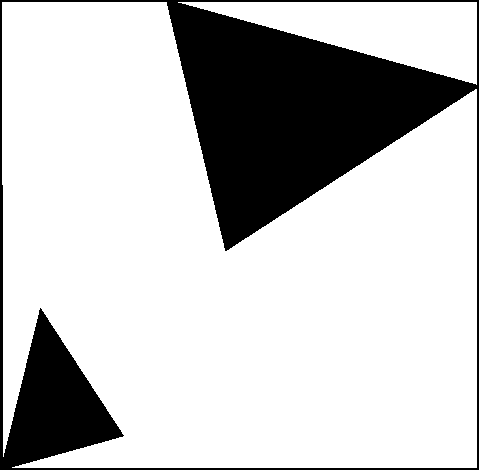
\includegraphics[width=0.5\textwidth]{aabb.pdf}
		\caption{Two-dimensional bounding box for two triangles}
		\label{fig:aabb}
	\end{center}
\end{figure}

A data structure we will be using frequently is minimum bounding boxes. A minimum bounding box for a set of geometric primitives is defined as the box with a certain smallest measure, that contains every single primitive in the set. While path tracing, these boxes can be two- or three-dimensional, making their respective measures the area and the volume. Because many parts of the path-tracing algorithm operate on axis-aligned regions of space, it makes sense to use boxes, whose edges are parallel to the coordinate axes. These boxes are called axis-aligned bounding boxes (AABB) and we can see an example of it in Figure {\ref{fig:aabb}}. Note, that in this case we have a two-dimensional bounding box but it is not hard to imagine, that AABBs work the same way in higher dimensions. To combine two AABBs, we just need to take the minimum and the maximum for each dimension of the two AABBs.

\section{Bounding Volume Hierarchies}
\label{sec:preliminaries:bvh}

Acceleration data structures are mandatory for path tracers. They reduce the amount of ray-primitive intersection tests to logarithmic in the number of primitives. The two main approaches are to either split the room among the space or to choose a particular number of primitives and wrap a bounding box around these primitives so when we intersect a ray with the scene only specific sets of primitives need to be tested for intersections. The acceleration data structure used in PBRT, the framework renderer we used, is the bounding volume hierarchy (BVH). It uses the latter approach. \cite{PBRT}

An example to partition the space would be kd-trees that splits the space parallel to one of the axis in each step. Those two sets of primitives are split recursively again until every leaf has only a maximum amount of primitives.  While kd-trees offer slightly faster ray intersection tests than BVH, their disadvantages outweigh. BVHs can be built much faster and are generally more numerically robust, so it is less likely to happen to miss intersection due to round-off errors than kd-trees are. Other desired traits of BVHs are that they require a maximum number of $2n - 1$ nodes for n primitives and, since we are partitioning the primitives, we will never have the same primitive in two different nodes which can happen in kd-trees. \cite{PBRT}

\begin{figure}
	\begin{center}
		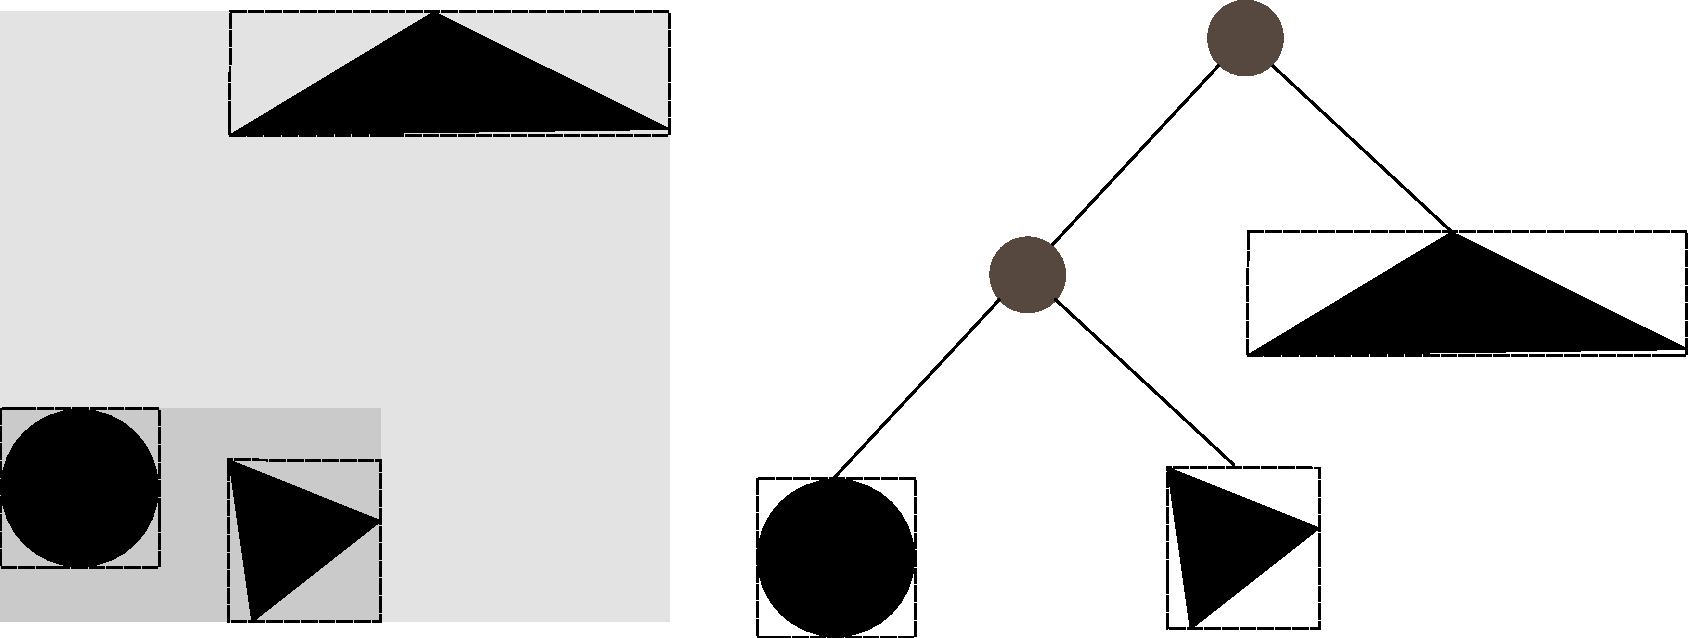
\includegraphics[width=0.9\textwidth]{bvh.pdf}
		\caption{On the left side the geometric representation of the primitives in the room and on the right side the representation in the BVH}
		\label{fig:bvh}
	\end{center}
\end{figure}


\subsection{BVH Construction}
\label{subs:const}

Obviously, the first step is the construction of the BVH data structure. The basic structure of BVH is a binary tree, with every node containing pointers to two children and every leaf holding a set maximum number of primitives. The construction technique that is most popular and also used in PBRT is the top-down construction. At the beginning of the construction we hold a set containing every single primitive of the scene. With each step, according to a split method we have chosen, we partition the primitives into two disjointed sets. Note that regardless of the split method we chose, we will always split the primitives among a certain axis to retain locality. Examples for popular splitting heuristics are "Middle", which just partitions the room among the middle of a chosen axis, "EqualCounts", which partitions the primitives among a chosen axis so the disjointed sets have the same number of primitives, and SAH (Figure \ref{pre:sah}). While the first two split methods allow a easy and fast construction, their quality is very lacking. Recursively splitting the root into two disjointed sets of primitives constructs the tree. When a certain node holds less than a defined number of primitives, we do not split again and instead call the node a leaf.

Every node needs to be holding onto some information in order to allow the intersection tests. Evidently, every inner node needs to have a reference to both of its children. As we have mentioned earlier, it also needs to store its bounding volume that wraps around all its primitives. When testing if we need to intersect any of the primitives of a node with a ray, we will be instead intersect the box with the ray. Typically, we will be using minimum fit axis-aligned bounding boxes for this task.

\subsubsection{Surface Area Heuristics}
\label{pre:sah}

\begin{figure}
	\begin{center}
		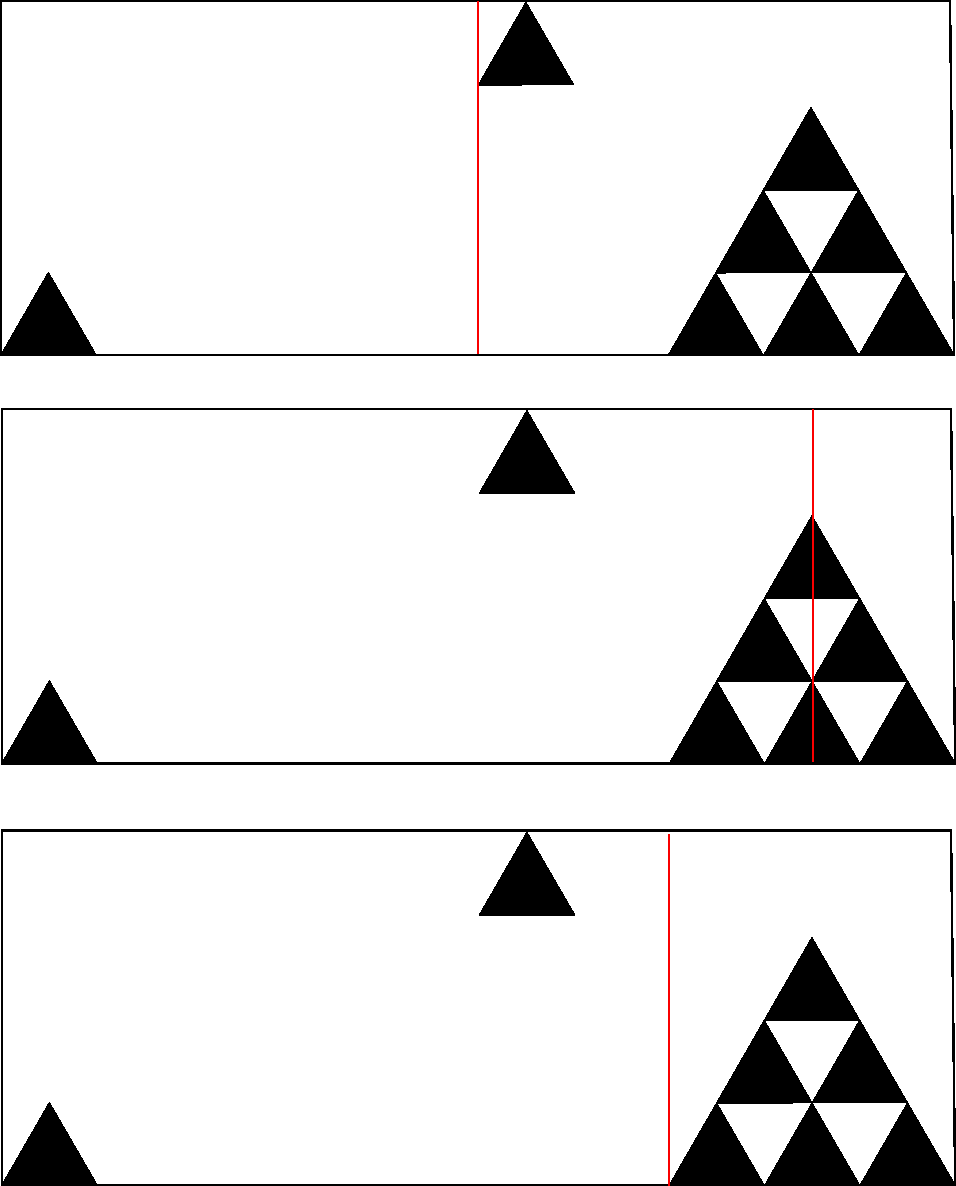
\includegraphics[width=0.5\textwidth]{sah.pdf}
		\caption{Three different split strategies: "Middle" in the top, "EqualCounts" in the middle and SAH in the bottom}
		\label{fig:sah}
	\end{center}
\end{figure}


We have presented two split methods in subsection \ref{subs:const}. While they both do work well in some situations, they both have clear disadvantages, especially if the primitives are not evenly distributed over the scene. Looking at Figure \ref{fig:sah}, it is obvious, that both the "Middle" and "EqualCounts" split the scene in a way that can lead to very inefficient intersection tests. In the "Middle" split, although the triangle mesh on the right child node are focused on a very small space, the drawn ray will still make intersection test with each of the triangles of the right child node. Similarly, in the "EqualCounts" split, many unnecessary intersection tests are made. A desirable split would be the third split and we will now introduce a split method that favors these kinds of splits.

The surface area heuristics (SAH) defines a model that assigns a quality to a given split. The idea behind the SAH cost model is actually very simple. When we want to decide the best possible split for given primitives, first, we have to decide if it is perhaps better not to split at all. That means, when a ray traverses through the bounding box of the node, we would have to make an ray-primitive intersection test with each primitive. That means the cost $c_g$ is 

\begin{equation}
\sum_{i = 1}^{N}t_{isect}(i),
\end{equation}

where N is the number of primitives and $t_{isect}(i)$ the time required for the intersection test with the i-th primitive. For simplicity, we will assume, that every ray-primitive intersection test takes the same amount of time.

Clearly, we can also split the primitives. The cost $c(A,B)$ would be

\begin{equation}
c(A,B) = t_{trav} + p_A\sum_{i=1}^{N_A}t_{isect}(a_i) + p_B\sum_{j=1}^{N_B}t_{isect}(b_j)
\end{equation}

with $t_{trav}$ being the additional overhead time to traverse through a child, $p_A$ and $p_B$ being the probabilities that the ray passes through the respective child node if we assume that the rays are evenly distributed in the scene. The probabilities $p_A$ and $p_B$ can be calculated using their respective surface areas:

\begin{equation}
p_C = \frac{s_C}{s_G},
\end{equation}

where $s_G$ is the surface area of the node and $s_C$ is the surface area of the child. This equation is the SAH.

Compared to the other two split strategies we presented, SAH actually adapts to the given geometry and tries to minimize the amount of ray-primitive intersection tests when traversing the tree. Therefore, SAH is much more versatile and performs better in most scenes.

\subsection{BVH Traversal}

Since the traversal of the bounding volume hierarchy is not relevant for this thesis, we will only give a short introduction of the general idea of it. If the reader is interested and would like to study additional readings about this subject, we would recommend the book "Physically Based Rendering" by Pharr, Jakob and Humphreys. \Cite{PBR}

We have constructed our BVH as an acceleration data structure for ray-primitive intersection tests now. In the next step, we will be intersecting rays that are tracked in out path tracing algorithm, with the BVH. First, we will be intersecting the given ray with the root of our tree. If there is an intersection between the bounding volume of the current node and the ray, we will be further checking for intersections of the ray with the children of our current node. If we arrive at a leaf node that contain primitives, we will make ray-primitive intersection tests with every primitive in the node. Note, that we can stop after we have found the first actual interaction with a primitive and have asserted that any other intersection of the scene with the ray is further away than the intersection we already found.  This way, we avoid many unneeded ray-primitive intersection tests 
and save a lot of time.

\section{Path Tracing Basics}
\label{sec:preliminaries:pat}

In this section we will discuss some of the basics of path tracing. It was first introduced in 1986 by James Kajiya in the proceedings of SIGGRAPH '86 \cite{JTK}. The general idea is to generate paths along the scene that start at the camera and end at a light source of the scene. In the beginning, we will be spawning rays that start at the point of the camera. Each of these rays will gather the color at the respective pixel they represent. At the intersection of the ray with the scene, we will be evaluating the rendering equation we have mentioned earlier:

\begin{equation}
L_o(p, \omega_o, \omega_i) = \int_{\Omega}f(p, \omega_o, \omega_i)L_d(p, \omega_i)|cos\theta_i|d\omega_i.
\end{equation}

We have noticed earlier, that this problem is a infinite-dimensional problem. That is because in order to calculate the color at the point we hit, we have to evaluate this equation for different directions $\omega_i$ according to the Monte Carlo integration. The reason for that is, as we have acknowledged earlier, it is impossible to calculate the result of this integral analytically. Instead, we will be sampling directions according to multiple distribution functions and estimate the contribution of these directions. The
ore, we have to spawn rays that will hit another point in the scene. As the result, we will get more light transport equations that need to be evaluated. To render the perfect image with path tracing, we could not stop after a finite number of steps, but in practice, we will break after a certain number of bounces or after the contribution of the point would be too low to actually change the image for the human eye. Instead, we will connect the current point with a sampled light source and finish the path. Such a path can be seen in Figure \ref{fig:path}.

\begin{figure}
	\begin{center}
		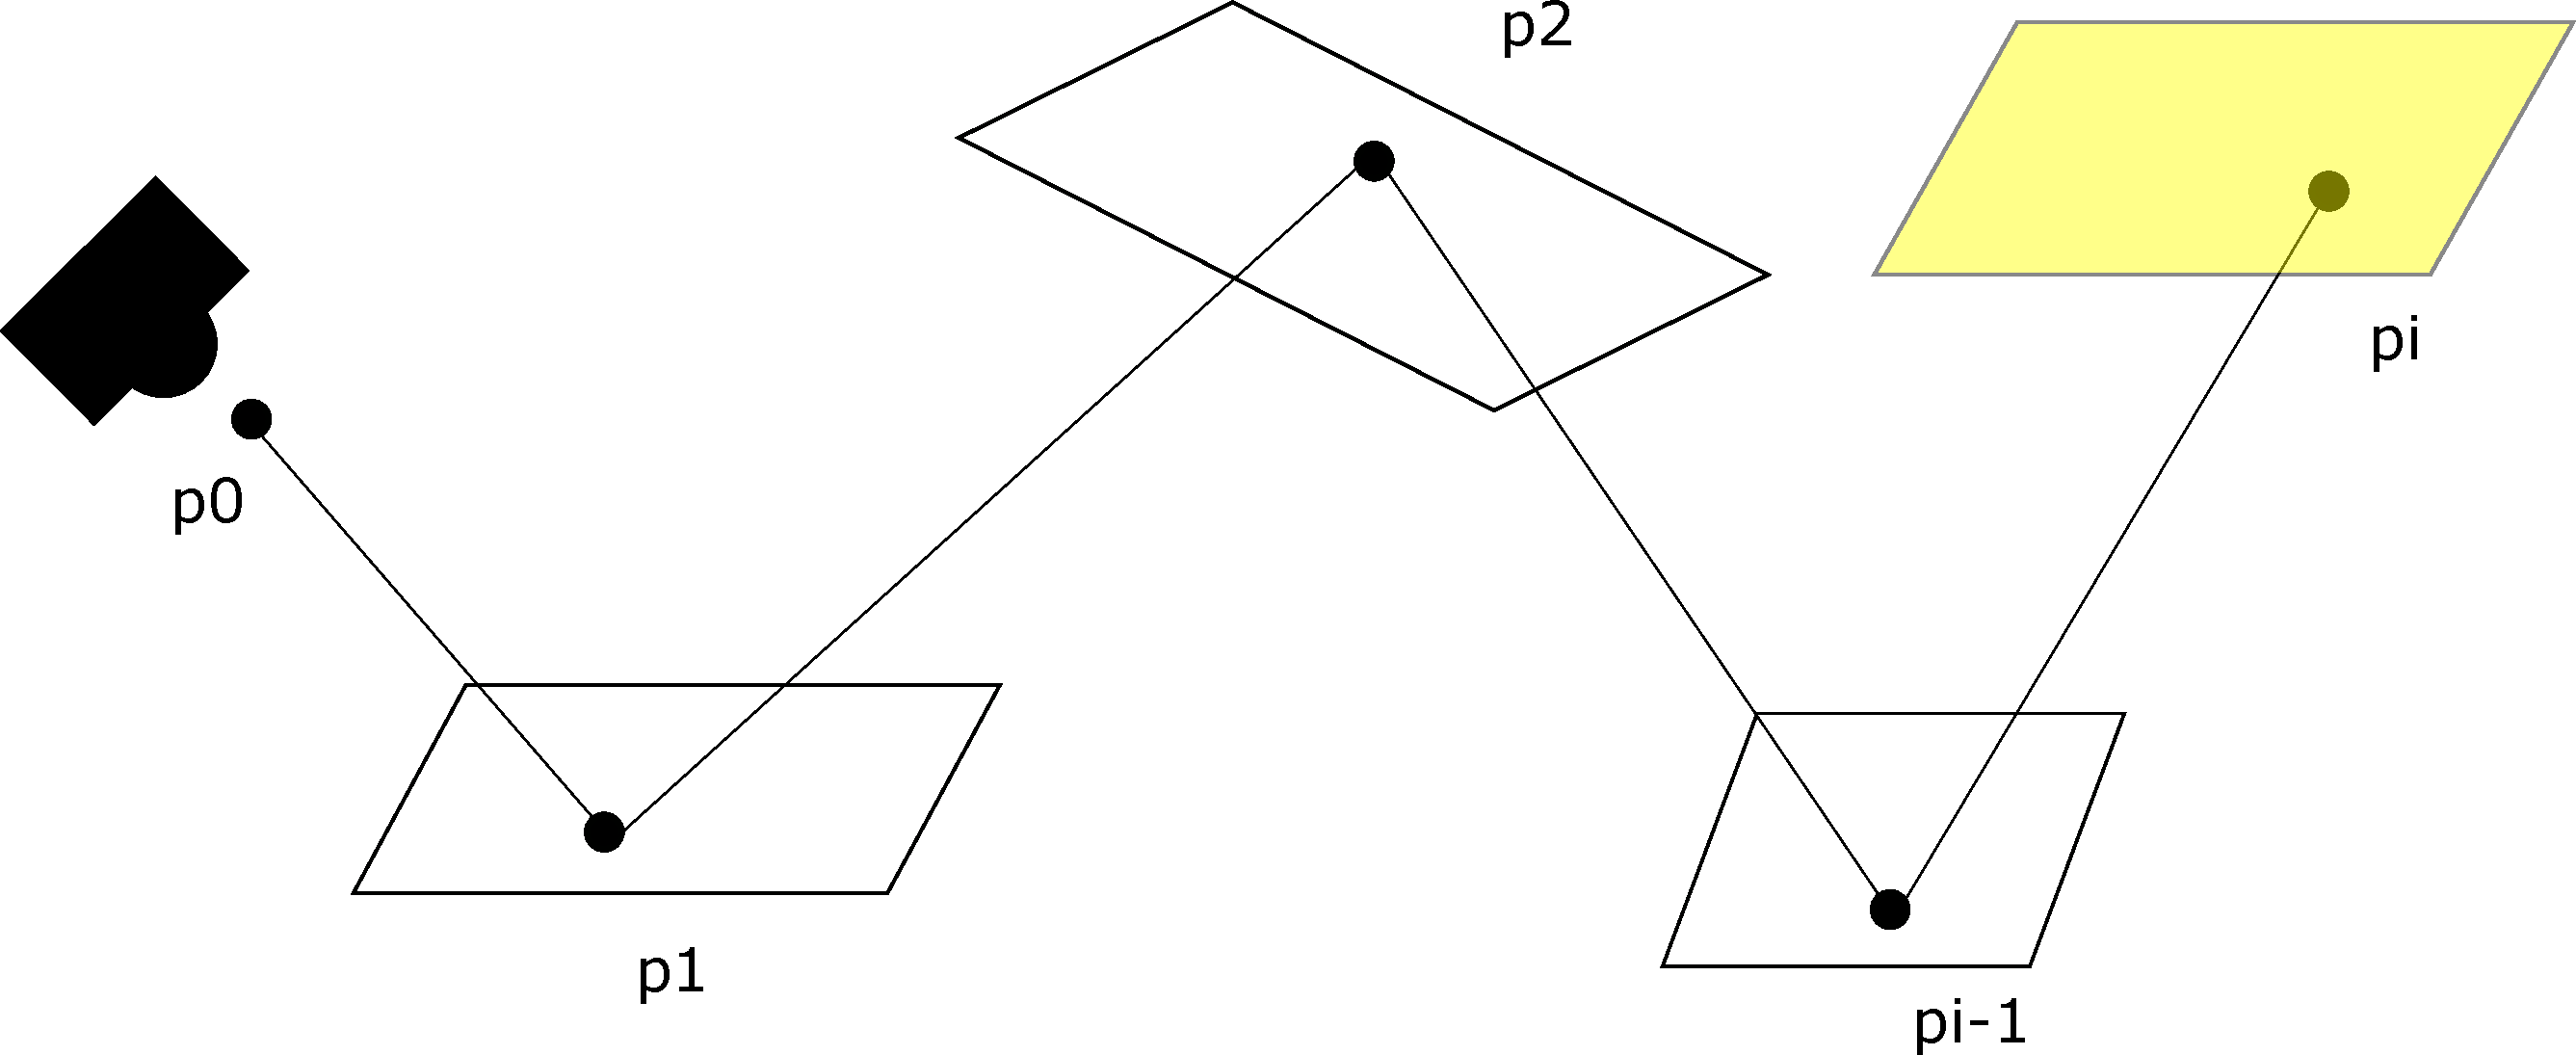
\includegraphics[width=0.7\textwidth]{path.pdf}
		\caption{A typical path for the path tracer starting at the camera and sampling a light source as the last vertex.}
		\label{fig:path}
	\end{center}
\end{figure}

We have already acknowledged the importance of using a sampling distribution that has a similar form to the functions of the integrand, when using Monte Carlo integration. In our light transport equation, we have two different functions. $f(p, \omega_o, \omega_i)$ is defined by the bidirectional scattering distribution function (BSDF) of the material of the point, basically a function that defines how the material reflects incident lighting, and consequently, we can use a distribution function similar to it to sample the directions $\omega_i$. The other function is the contribution of the light sources for the point $L_d(p, \omega_i)$. The sampling distribution needed to importance sample this function would be a distribution that reflects the amount of incident lighting from a given direction $\omega_i$. Now, suppose we have a situation where the scene has a substantial number of light sources, say 10.000 or even one million light sources. In this case, it would take a great time to estimate this distribution. In this thesis, our goal is to deal with these kinds of scenes with a gigantic number of light sources by creating an accelerator data structure, the light bounding volume hierarchy. This data structure importance samples a light given the intersection point that can be then used to estimate the light transport equation.